\documentclass[conference]{IEEEtran}
\usepackage[T1]{fontenc}
\usepackage{times}
\usepackage{amsmath,amssymb}
\usepackage{graphicx}
\usepackage{booktabs}
\usepackage[numbers,sort&compress]{natbib}
\usepackage[hidelinks]{hyperref}
\hypersetup{pdftitle={When Is Robot Recovery Justified? Decision-Sufficient Explanations and the Limits of Observation},pdfauthor={},pdfsubject={Anonymous full research manuscript},pdfkeywords={}}
\newcommand{\Good}{\operatorname{Good}}
\newcommand{\supp}{\operatorname{supp}}
\title{When Is Robot Recovery Justified?\\Decision-Sufficient Explanations and the Limits of Observation}
\author{Anonymous Authors}
\begin{document}
\maketitle
\begin{abstract}
An effective recovery skill need not be justifiable from available observations, and a finite pure rule need not be statistically deployable. Decision-Sufficient Recovery Explanations (DSRE) provide minimum observable action facts or constructive observation, repertoire and reference-insufficiency witnesses. Established sufficient-rule and selective-risk principles supply the mathematical core. A preserved 333-parent prospective cohort confirmed a PickCube justification-coverage gain, mostly on already-successful starts, while strict PushCube routing always abstained. A separately preregistered operational study completed 360/360 independent calibration parents. Pick continue and Push recover each incurred one erroneous assigned parent in 180; simultaneous upper error bounds are 5.19\%, below the 10\% target. Rare Pick recovery remains unqualified. The first selected-execution prefix check halted the new test at 0/160 complete parents, so held-out operational effects are not estimable. We preserve that failure and report matched retrospective comparisons and a fixed offline corruption study separately. Ordinary rules remain equivalent; meaningful third-task recovery validation is blocked. The result characterizes intervention justification and its limits, without a new controller, algorithmic superiority or a completed operational validation claim.
\end{abstract}

\section{Introduction}
A robot choosing between continuing a manipulation and invoking recovery faces three different situations: either skill may succeed, recovery alone may succeed, or neither skill may succeed. The same declared observations can describe all three. Explaining a policy's prediction does not establish that its selected intervention is adequate, and a high average recovery success rate does not resolve an ambiguous individual decision.

Table~\ref{tab:physical} makes the problem concrete. Two PickCube checkpoints share six primary predicates, but one is recover-only and the other neither-success. A signed geometric predicate separates them without making the inadequate state recoverable. A PushCube pair has opposing adequate actions yet identical values under the entire declared vocabulary. A both-success checkpoint, by contrast, can support an adequate action without establishing that recovery was necessary.

We ask: \emph{What observable evidence suffices to justify a fixed robot recovery intervention relative to measured paired outcomes, and what explains insufficiency?} The operational contribution joins minimum observable action facts, constructive observation/repertoire/reference witnesses, and a finite development-time instrumentation frontier under one explicit intervention contract. Established sufficient-rule and robust-intersection principles supply the reasoning. We evaluate their robotics consequences against equally informed rules and trees, rather than claiming a new enumeration algorithm.

Our evidence separates exact finite-reference statements, exploratory grouped cross-fitting, an interrupted preliminary cohort, and a separately preregistered untouched suffix. The key distinction is between increased successful justification coverage and increased justified recovery where recovery is required. The same measured four-category outcomes support this decomposition without changing the solver, utility, or hypothesis after seeing results.

\section{Related Work and Scope of the Contribution}
Minimal sufficient explanations for factored MDPs already justify decisions using reward and occupancy structure~\cite{khan2009}. Anchors target high conditional precision for a predictor under a perturbation distribution~\cite{anchors}; probabilistic sufficient explanations likewise concern preservation of model decisions~\cite{pse}. DSRE instead labels reference states with measured adequacy of two interventions. This changes the target of explanation, not the established idea of sufficient evidence.

Outcome-aware subgroup rules are also established. DISCRET synthesizes rules for treatment-effect estimation~\cite{discret}; our exact risk-aware rule comparator shares the principle of matching observable subgroups to outcomes, without purporting to reproduce its learned synthesis. More fundamentally, robust action intersection under partial observability already covers our strict feasibility criterion~\cite{partial}. Our refinement proposition is an elementary specialization of that principle. We claim no new theorem of partial observability, hitting-set optimization, pure-rule enumeration, or calibration.

Robot recovery research includes corrective actions from violated preconditions in CAPE~\cite{cape} and decision-tree monitoring with recovery under decision uncertainty~\cite{peddi}. Explicit observation of decision context is developed by Ernst et al.~\cite{ernst}. DA-GRD studies grasp-relevant ambiguity reduction through physical sensing~\cite{dagrd}, whereas our optional channels are fixed Boolean summaries of already available simulated poses. RESCUE evaluates alarms through matched counterfactual interventions~\cite{rescue}; we do not claim to introduce intervention-relative evaluation or state branching. The latter two works are cited as preprints. Our narrower contribution is an executable, intervention-grounded sufficiency analysis with distinct obstruction witnesses, equal-information controls, and a measured characterization of its limits. The formulation makes intervention adequacy, missing observations, inadequate skills, and missing reference support separately testable.

Selective classification already formalizes rejection, risk--coverage tradeoffs and high-probability risk control~\cite{selective2017}. Our independent binomial gate and abstention semantics use these established ideas. The contribution is not a new reject-option or calibration algorithm: it is the robotics contract joining measured intervention adequacy, finite witnesses, statistical action eligibility and explicit completion loss when evidence is insufficient.

\section{Decision-Sufficient Recovery Evidence}
\subsection{Reference model and observable inputs}
Let $s$ be a full robot--environment state and $x=F(s)$ its predecision observation signature, possibly including a timestamped earlier observation. The fixed actions are $\mathcal A=\{c,r\}$: continue and recover. Executing skill $a$ for the declared horizon gives terminal binary utility $U(s,a)$. The measured reference $R$ contains paired outcomes and independent parent identifiers. Define
\begin{equation}
\Good(s)=\{a\in\mathcal A:U(s,a)=1\}.
\end{equation}
Adequacy is $a\in\Good(s)$, not positive treatment effect. Both actions may be adequate; neither may be. Choosing continue from an already successful state can maintain success, but cannot be counted as a newly recovered failure. Regret relative to the best available action differs from inadequacy: a neither-success state has no successful alternative but still makes a chosen action unacceptable under our adequacy definition.

For known literals $E\subseteq x$, let $M_R(E,x)$ contain all reference rows not contradicted by $E$. An UNKNOWN reference predicate remains compatible; an unknown query value cannot be asserted as a literal. A strict finite-reference justification is $(E,a)$ satisfying
\begin{equation}
\begin{gathered}
|\{\text{parent}(s):s\in M_R(E,x)\}|\ge 2,\\
a\in\bigcap_{s\in M_R(E,x)}\Good(s).
\end{gathered}
\label{eq:strict}
\end{equation}
Missing or unqualified outcomes prevent a certificate. The task, skills, horizon, observation map and outcome definition must match the reference scope. Nonempty support prevents vacuous justification, while two independent parents are an explicit reference-support requirement, not a statistical confidence guarantee.

DSRE searches all subsets of known literals for minimum $|E|$. Canonical ties prefer larger row support, then continue, then lexicographic facts. A necessary-literal witness is a compatible row that makes the selected action inadequate when that literal is removed. Minimum cardinality guarantees such a counterexample under the fixed support rule: removing a literal expands support and cannot reduce its parent count. The certificate records scope, matched rows, measured outcomes and reference identity. It says nothing universal about unobserved states.

\begin{table*}[t]
\caption{Measured physical cases from the qualified development reference. The six-bit primary signature follows the predicate order in Sec.~IV; L tests whether object.x minus goal.x is below -0.02 m. Outcomes are terminal success after the fixed continuation/recovery horizon. A/B share primary predicate values but differ in L; B remains inadequate. D/E have opposing adequate actions and identical signatures under all twelve declared predicates. Case C illustrates adequacy without action necessity. Internal identifiers and source hashes are retained outside the anonymous paper.}
\label{tab:physical}\centering
\begin{tabular}{clrrrrc}\toprule
Case & Task & Time (s) & Object.x$-$goal.x (m) & Primary bits & $L$ & Continue / recover\\\midrule
A & Pick & 3.50 & -0.03401 & 001111 & T & 0 / 1\\
B & Pick & 3.50 & +0.05460 & 001111 & F & 0 / 0\\
C & Pick & 4.50 & -0.00023 & 111110 & F & 1 / 1\\
D & Push & 2.65 & -0.14386 & 011110 & T & 0 / 1\\
E & Push & 2.65 & -0.14476 & 011110 & T & 1 / 0\\
\bottomrule\end{tabular}
\end{table*}

\subsection{Why justification fails}
After strict search abstains, DSRE returns all applicable scoped obstructions. \emph{Repertoire inadequacy}: a compatible qualified state has $\Good=\varnothing$. \emph{Observational ambiguity}: compatible states have disjoint nonempty adequate-action sets; with two actions, a continue-only and a recover-only state suffice. \emph{Reference insufficiency}: support is too small, outcomes are missing/unqualified, or scope is inconsistent. A support shortage is not proof of physical impossibility. Why-not witnesses show a failing compatible reference row for each candidate action; they do not assert that the current unknown state is that row.

For example, two PickCube checkpoints share all six primary predicates. At one, object.x$=-.04661$ m and goal.x$=-.01260$ m; continue fails and recover succeeds. At the other, object.x$=.03920$ m and goal.x$=-.01540$ m; neither succeeds. The extra predicate object.x$-$goal.x$<-.02$ separates them and gives the first a pure recovery child supported by two parents in the full reference. It leaves the second inadequate. The minimum recovery certificate needs three facts: goal not near, progress, and object left of goal. It matches five reference parents, so exact-signature support differs from support of the minimum rule. Such small support is fragile when parents are held out. In PushCube, a recover-only and a continue-only checkpoint share all twelve declared predicates despite different raw poses. No channel in this menu separates them. This is a vocabulary limitation, not an impossibility claim for arbitrary sensors or raw-coordinate reasoning.

\subsection{Observation refinement and known equivalence}
For complete observed signatures, partition $R$ into classes $Z$ and define the descriptive finite ceiling
\begin{equation}
 C_R(F)=\frac 1{|R|}\sum_Z |Z|\,\mathbb{I}\!\left[\bigcap_{s\in Z}\Good(s)\ne\varnothing\right].
\end{equation}
This exact-signature ceiling is distinct from supported conservative-rule coverage, particularly with UNKNOWN values. It is also distinct from performance on held-out states evaluated against a smaller training reference.

\noindent\textbf{Proposition (finite refinement).} For deterministic complete predicates on the same fixed reference, if $F'$ refines $F$, then $C_R(F')\ge C_R(F)$. Any neither-success row remains unjustifiable after arbitrary refinement.\newline
\emph{Proof.} Every child of an actionable class retains its common adequate action. A class containing a neither-success row has empty intersection for that row's child. Summing child masses proves the first statement; empty $\Good$ proves the second. $\square$

For $m=6$ optional unit-cost predicates, enumerate $J$ with $|J|\le b$, maximize training $C_R(F_0\cup J)$, then minimize cost and use canonical channel ties. This is offline instrumentation design, not online active sensing. The budget counts predicates, not physical sensors, latency or energy. With $d$ known query facts and $n$ reference rows, direct strict search costs $O(n d 2^d)$ and memory can be bounded by cached bit masks. Channel selection considers at most $2^m$ menus. These small exact searches are practical here, without implying scalability to arbitrary vocabularies.

B7, exhaustive zero-error outcome-aware rules with identical support and ties, is mathematically identical to DSRE. Two-literal rules are a restricted grammar; risk-aware B5 allows empirical error at most $.1$ and is provisional, not strict. An exact rule's name or witness format does not constitute an algorithmic advantage. Adding predicates preserves old rules on a fixed table, but neither cross-fit performance nor a selector choosing nonnested menus must improve monotonically.

\begin{figure*}[t]
\centering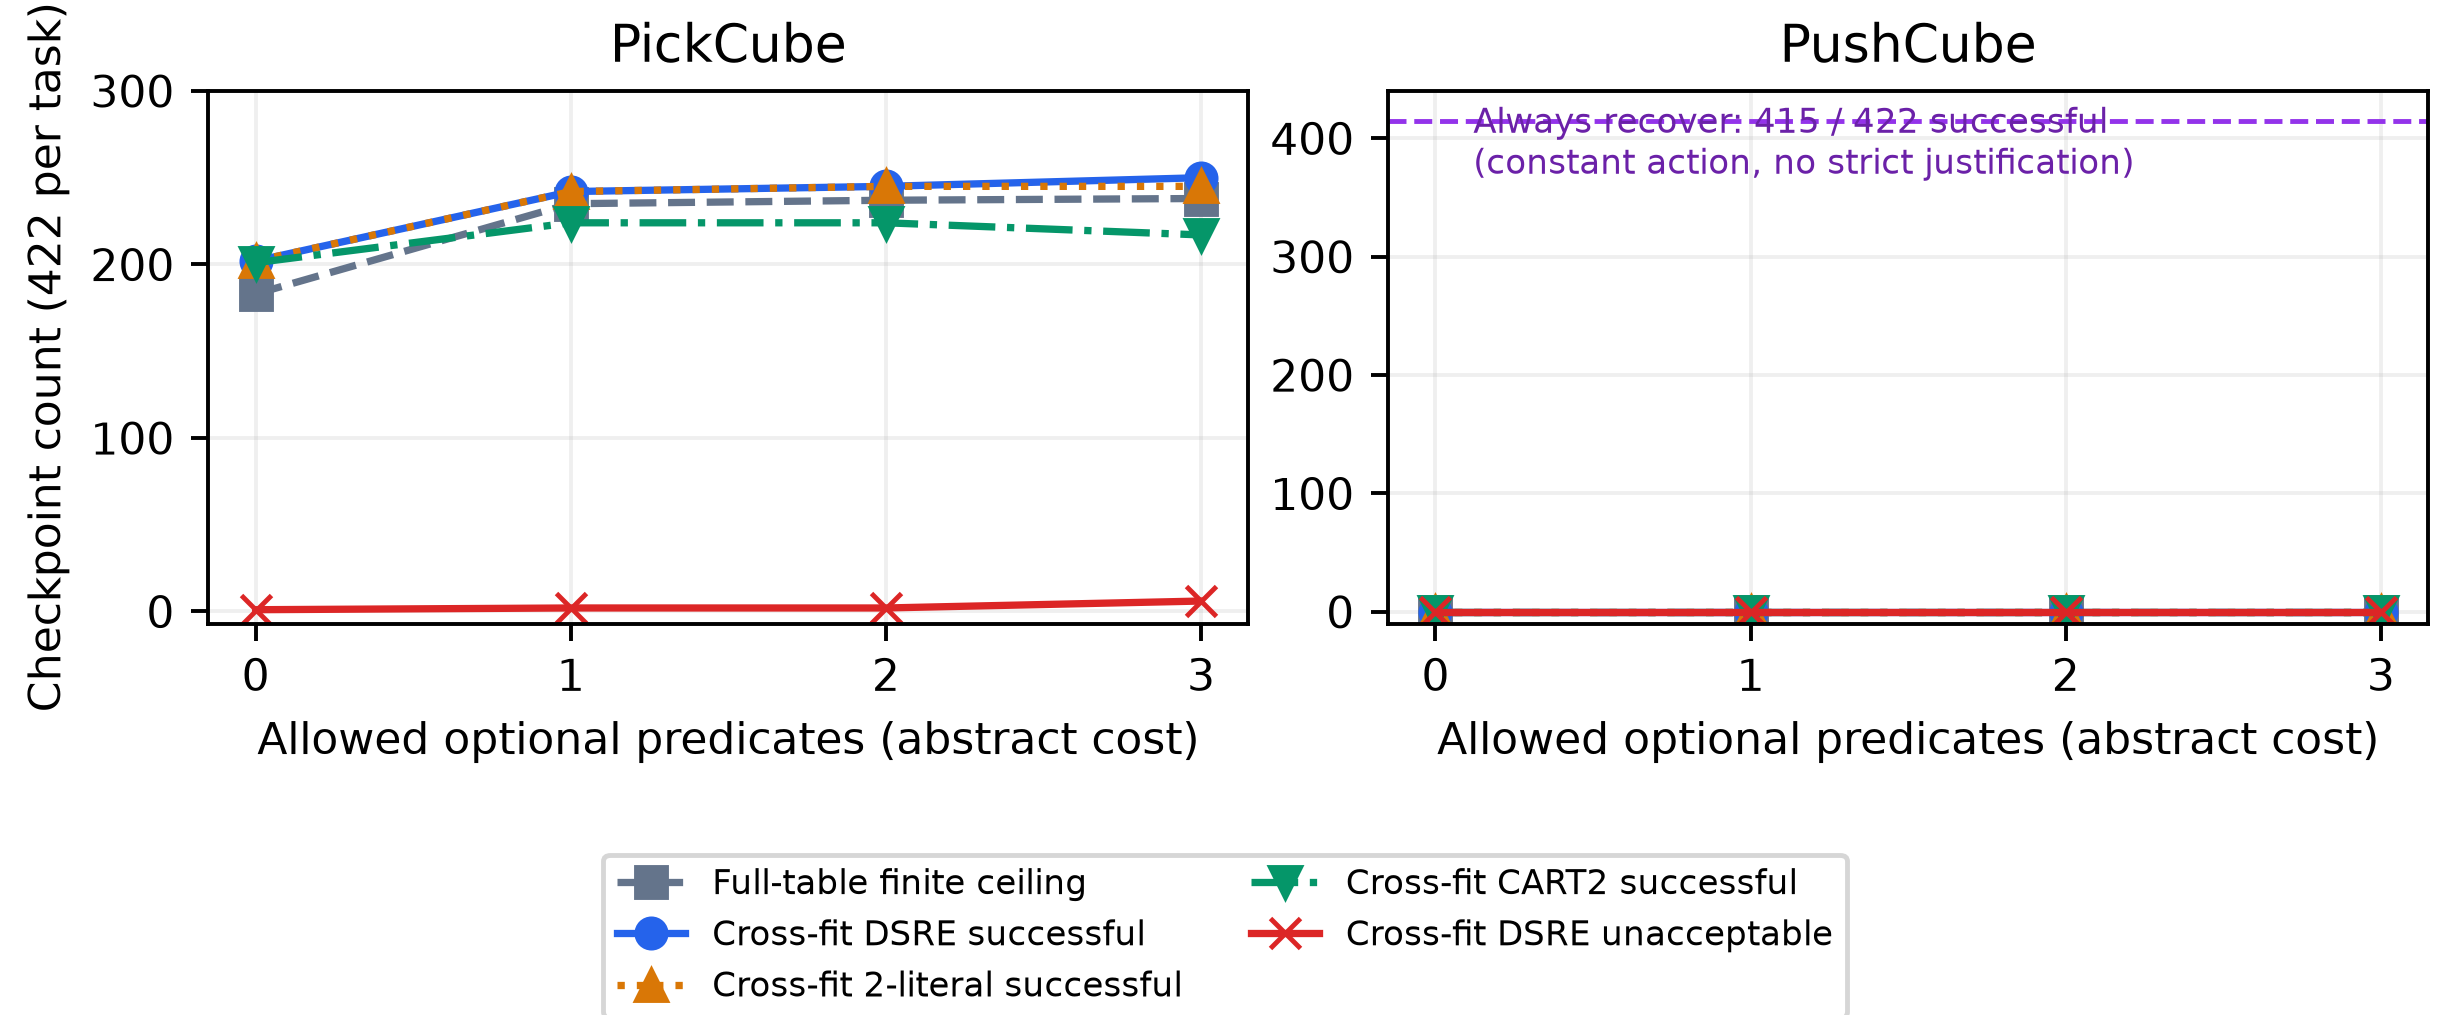
\includegraphics[width=\textwidth]{figures/frontier.png}
\caption{Finite-reference ceilings and exploratory grouped cross-fit outcomes are different estimands, each with 422 checkpoints/task. A cross-fit recommendation can exceed full-table actionable mass because its training reference omits conflicting held-out rows; that does not violate the refinement proposition. Cost counts optional Boolean pose predicates. PushCube strict curves coincide at zero. The two-literal control equals DSRE through b2; b3 gains include additional unacceptable choices.}
\label{fig:frontier}
\end{figure*}


\section{Operational Assurance Under Finite Data}
\subsection{A fixed router and explicit deferral}
A minimum sufficient rule does not itself specify what the robot does when evidence is insufficient. We make this operational: the router emits continue, recover, or defer/stop. Deferral contributes zero to autonomous completion. Conditional success among acted-on checkpoints and unconditional autonomous completion therefore answer different questions. We report both, rather than implicitly executing the best alternative after abstention. Initially successful states, genuinely failed starts and the four paired outcome categories remain separate.

The fixed risk-tier candidate is the existing strict-then-provisional router: retain a strict DSRE recommendation when available; otherwise consult an ordinary two-literal outcome-aware rule with empirical error at most $.10$. The proposal is not automatically authorized. An independent statistical gate may remove an action but never choose a new action using its test outcome. The same grammar and ties give an identical ordinary B7-then-risk router; this is an explicit equivalence, not an algorithmic improvement. Frozen one-/two-literal rules, four-outcome CART, a fixed support-pruned tree, B5, constant actions and a greedy pure-rule control use the same predecision facts. A full-signature selector is an upper-information control, while policy-faithful rules explain a frozen tree's label without certifying its intervention adequacy.

\subsection{Independent parent-action risk}
Let $I_{g,a}$ indicate that frozen router $\pi$ assigns action $a$ to at least one of the two registered conditions of independent seed parent $g$. Define $V_{g,a}$ as one if any such assigned condition is unacceptable. Our statistical target is
\begin{equation}
 p_{t,a}=\Pr(V_{g,a}=1\mid I_{g,a}=1,\,t),
 \qquad p_{t,a}\le .10.
\end{equation}
This is a parent-action any-error probability under the declared seeded task distribution. It is not an arbitrary-time or checkpoint-weighted safety claim. Conditions within a parent are never counted as independent calibration samples. With $k$ erroneous assigned parents among $n$ assigned parents, the classical one-sided exact binomial upper bound is
\begin{equation}
 U(k,n;\delta)=\begin{cases}
 1,&n=0\text{ or }k=n,\\
 B^{-1}_{k+1,n-k}(1-\delta),&\text{otherwise}.
 \end{cases}
\end{equation}
Here $B_{u,v}$ is the Beta CDF. The binomial interpretation assumes independent seed-parent draws from the declared simulator distribution; grouping conditions alone does not establish that distributional assumption. This is established Clopper--Pearson inference~\cite{clopper1934}, not a DSRE theorem. Models, rules, thresholds, support, ties, strata and outcome semantics are fixed before calibration. For 17 fixed methods and four task/action strata, all formal gates use $\delta=.05/(4\cdot 17)$, protecting the family with Bonferroni. The primary four-stratum diagnostic at $.0125$ is also reported but never overrides this stricter gate. Zero errors require 69 assigned parents for the global gate, compared with 42 for the four-stratum diagnostic. An empty or underpowered stratum is NOT CERTIFIED.

A proposed action is enabled only when its own stratum passes. The completed calibration decision is sealed before any test parent; test labels cannot change it. The resulting assurance is distribution- and input-model-specific, not a deployment guarantee for hardware, noisy sensing or altered controllers. A short finite certificate and a statistical authorization are distinct proof obligations. An initially inadequate repertoire cannot be repaired by observing more facts, and an underpowered action cannot inherit calibration from another action's large sample.

\subsection{Predeclared imperfections and input cost}
An offline sensitivity study corrupts only recorded predecision observations, leaving measured paired outcomes unchanged. The fixed grid includes unavailable selected facts, missing earlier history or pose, Gaussian pose noise at 1 and 5 mm with three fixed replicates, and actual prefix pose delays of 50 and 250 ms. Every comparator receives the same corrupted packet. UNKNOWN is not a negation. States within 1 mm of a declared predicate boundary form a predeclared subgroup. We measure action/certificate stability, factual contradictions, inadequate actions and deferral. Clean statistical authorization is not transferred to corrupted inputs. Serialized observation bytes, scalar fields and routing runtime describe the input/computation interface, not physical sensing latency, energy or cost.

\section{Hypotheses and Evaluation}
We test four fixed propositions: \textbf{H1}, observation refinement increases strict justification selectively; \textbf{H2}, increased justified coverage need not increase required recoveries; \textbf{H3}, finite-reference purity differs from independent statistical risk eligibility; \textbf{H4}, imperfect observations can change factual certificates, adequacy and deferral. These are tested hypotheses, not promises of positive findings. No hypothesis requires beating the equivalent B7 rule.

\subsection{Qualified reference and grouped reanalysis}
The experiments use ManiSkill 3~\cite{maniskill} on a CPU backend. The reference has 844 qualified checkpoint pairs, 422 per task and 211 independent seed parents per task, after 76 exclusions from 920 candidate checkpoints. Each parent contributes two registered conditions: nominal/2-cm offset for PickCube and nominal/misaligned for PushCube. Both unchanged skills run for 70 controls, or 3.5 s, and adequacy uses terminal task success. Pick recovery is a frozen staged regrasp (open/lift, approach, close, goal); Push recovery lifts and repositions behind the object before pushing. Continuations retain goal-directed Cartesian control. Prefix replay and controller memory are qualified; native snapshots are not trusted for branching. Paired deterministic outcomes describe this simulator protocol, not repeated-trial success probabilities.

The primary predicates are object--goal distance at most 0.03 m; hand--object distance at most 0.04 m; goal-distance reduction and object displacement from the first prefix packet each at least 0.005 m; summed absolute finger positions at most 0.04 m; and hand height above the object greater than 0.03 m. Optional predicates test object--goal x/y and hand--object x offsets below $-0.02$ m or above $0.02$ m. They summarize simulator-supplied poses, not validated real perception or newly acquired measurements. Privileged contact/grasp fields are excluded from primary queries.

We retain the original grouped five folds, holding both conditions of every seed together. Channel sets are selected on training parents only. All reference data have already informed development: this is exploratory cross-fitting, not untouched confirmation. We independently regenerate saved predictions, exact ceilings and error cases, and resample independent seed parents together for paired uncertainty. The paper reports counts and paired percentile intervals, not trajectory-row standard errors.

Equal-information controls include B7, one-/two-literal pure rules, outcome-aware CART depths 1--3, B5 at empirical error $.1$, a strict-first risk-aware wrapper, greedy coverage/entropy selectors, canonical/random menus and constant-action policies. Trees use four outcome classes and a shared two-parent inference gate. Controls that relax strictness are labeled provisional; their successes cannot be advertised as strict certificates.

\subsection{Independent prospective follow-up}
The original 400-parent schedule was interrupted by an unexplained SIGTERM after 133 qualified checkpoints; 132 from 66 complete parents (33/task) form its primary analysis, with one orphan excluded. Pick successful recommendations rose 29$\to$38/66, but failed-start successes stayed 6/20; strict CART2 matched all 264 preliminary decisions. These positive preliminary findings were inspected before authorizing a separate follow-up, so its primary estimator uses only the previously untouched suffix: 166 Pick and 167 Push parents, both original conditions. The incomplete Pick boundary parent is never remeasured. References, b0/b1 channels, support/ties, skills and tree nodes remain frozen; no models are retrained.

Each candidate action starts from a separate seeded reset followed by the full canonical action prefix. Every prefix state, endpoint, model edit and controller custom memory must match before intervention. Native snapshots are not used. Qualification checks restoration and recorded action equations; future trajectories are not independently duplicated. New physics is bounded to three cumulative hours in synchronous 5--8 minute chunks, with atomic completion after both conditions. Preregistered interrupted-parent exclusion and untouched-parent continuation prevent replacement or repeated measurements; qualification failures halt the study.

Primary suffix-only effects compare b1--b0 with 4000 paired seed-parent bootstrap draws, retaining both conditions together. Resampling all complete task parents also defines the initial-state and outcome-category contrasts. A separate completed-parent pool is descriptive only because the preliminary cohort was inspected. Neither study supplies independent deployment calibration.

\begin{figure*}[t]
\centering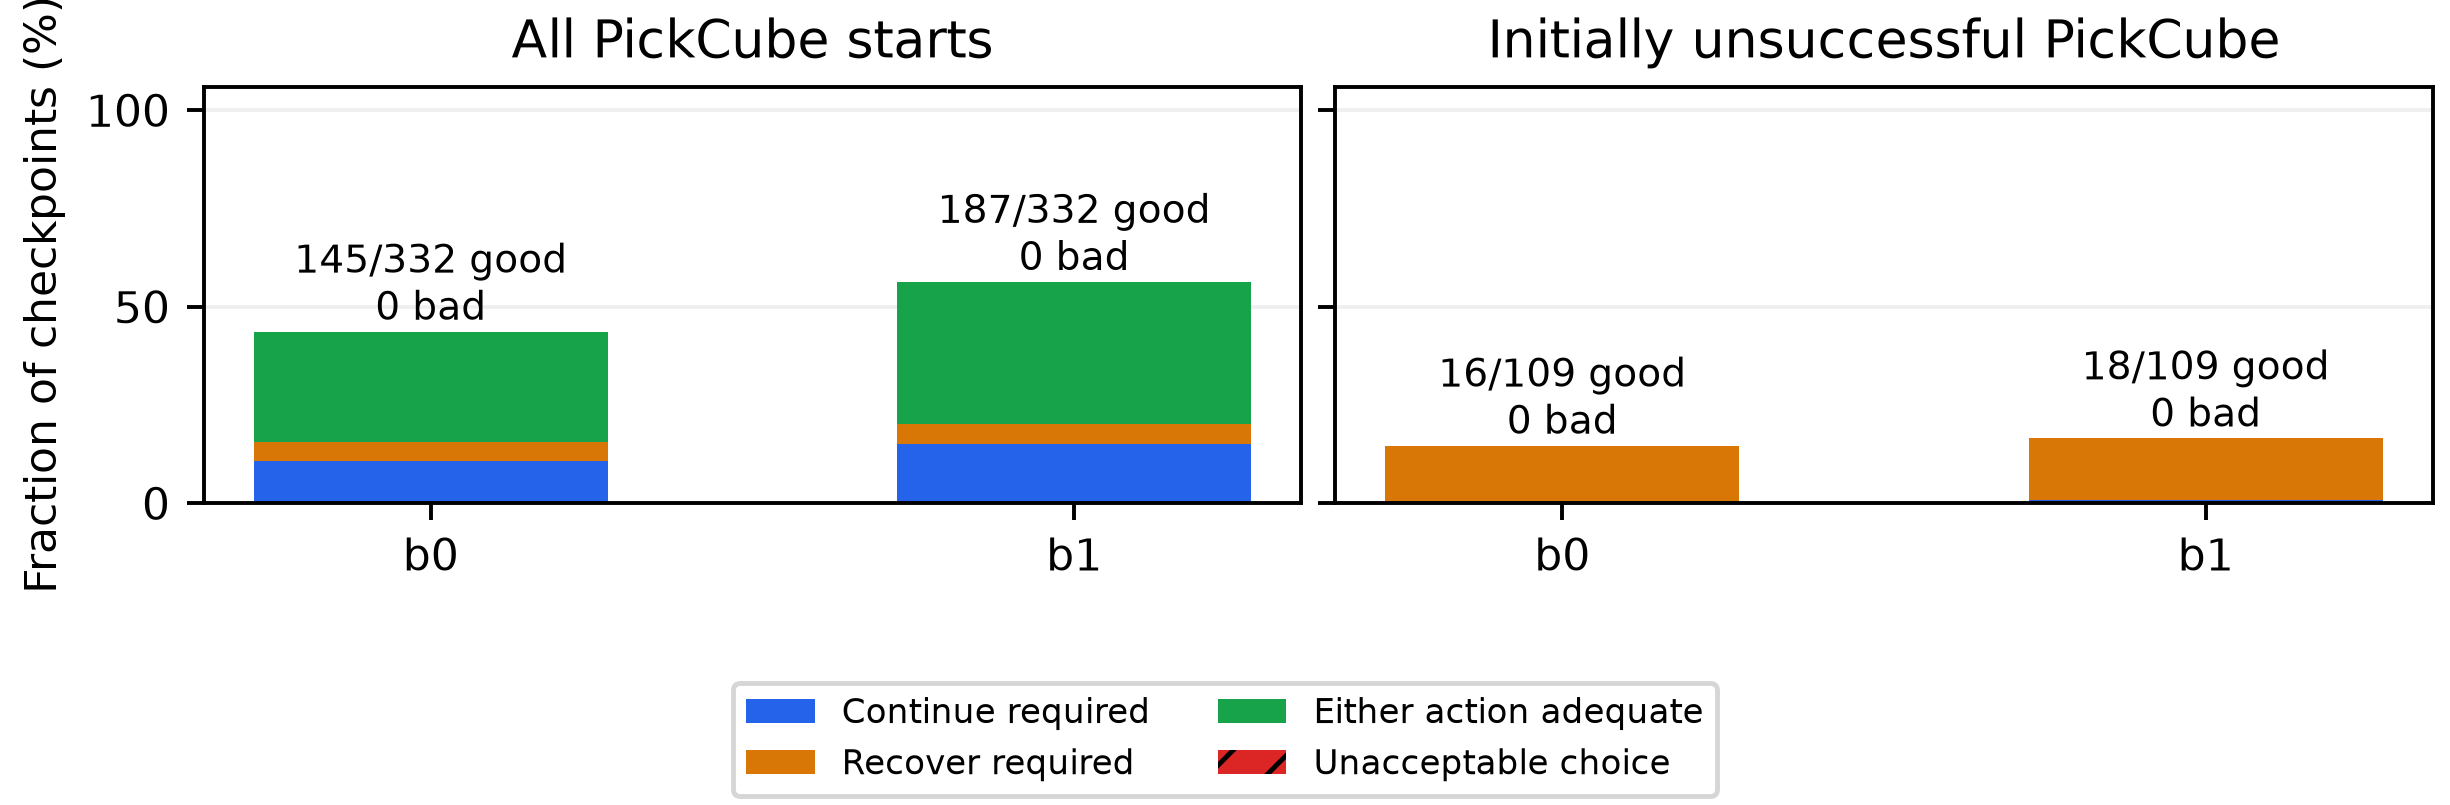
\includegraphics[width=\textwidth]{figures/necessity.png}
\caption{Untouched suffix-only PickCube outcomes under frozen strict-reference routing. Colors separate successful choices required relative to the two fixed skills from interchangeable choices when both succeed; red marks unacceptable choices. Denominators and failed-start outcomes are explicit. These are measured out-of-sample outcomes, not finite-reference ceilings or risk guarantees. Provisional empirical-risk controls use a different standard and are reported separately.}
\label{fig:necessity}
\end{figure*}

\section{Results and Their Boundaries}
\subsection{Finite reference and exploratory cross-fitting}
On the 422 development Pick checkpoints, finite actionable masses at budgets 0--3 are 183,235,237,238; all six optional predicates yield 248. Push remains zero throughout. These exact same-table statements support the selective observation effect (H1) and the repertoire boundary, not deployment ceilings. Figure~\ref{fig:frontier} distinguishes them from outcomes against smaller cross-fit training references.

Grouped Pick cross-fitting gives 202$\to$242 successful strict recommendations/422 at b1: +9.48 percentage points, paired 95\% interval[6.64,12.32], with unacceptable choices 1$\to$2. Among 145 failed starts, successes fall 19$\to$18. B7 matches all 16,880 registered decision/explanation views; pure two-literal rules match throughb 2. Strict CART2 gives 201,224,224,217 successful recommendations with one unacceptable choice each; provisional $.9$ CART2 gives 296/422 successes and one error at b0.

For Push, always recover succeeds 415/422 while strict coverage stays zero. Compatible reference classes include neither-success cases and opposing adequate actions; six conflict edges remain unseparated by all six optional predicates. This supports H3 without suggesting the recovery skill is ineffective. Held-out Pick errors include unseen neither-success outcomes and an absent b1 signature, illustrating the generalization boundary: training-pure rules can fail beyond their reference.

\subsection{Untouched suffix-only outcomes}
The follow-up completed 333/333 parents and 666/666 primary checkpoints; 0 parents are missing or partial. Its status is explicitly complete. The earlier 133 qualified checkpoints, including the orphan, remain unchanged and outside the suffix-only estimator. No seeds were substituted, no thresholds or models changed, and no significance criterion stopped sampling.

\begin{table}[t]
\caption{Suffix-only strict DSRE recommendations / successful / unacceptable. Denominators: Pick 332 checkpoints/166 parents; Push 334/167. Initially unsuccessful starts are separate.}
\label{tab:fresh}\centering
\begin{tabular}{lcrr}\toprule
Task & Budget & All starts & Failed-start good / starts\\\midrule
Pick & 0 & 145 / 145 / 0 & 16 / 109\\
Pick & 1 & 187 / 187 / 0 & 18 / 109\\
Push & 0 & 0 / 0 / 0 & 0 / 334\\
Push & 1 & 0 / 0 / 0 & 0 / 334\\
\bottomrule\end{tabular}
\end{table}

Pick b1--b0 successful strict coverage changes by +12.65 percentage points, paired 95\% interval $[9.33,16.27]$. Unacceptable choices are 0$\to$0; abstentions are 187$\to$145. Zero observed errors or a degenerate bootstrap interval would not establish zero population risk. Push strict successes are 0$\to$0/334, while always recovering succeeds 334/334.

Pick outcome classes (continue-only/recover-only/both/neither) contain 60/84/164/24 checkpoints. Push outcome classes (continue-only/recover-only/both/neither) contain 0/167/167/0 checkpoints.

\subsection{Decision necessity and strongest controls}
The Pick gain decomposes into +14 continue-only, +1 recover-only, +27 both-success and +0 neither-success choices (Fig.~\ref{fig:necessity}). Initially unsuccessful successes change 16$\to$18/109; additional successful required-recovery recommendations number +1. Failed-start coverage changes by +1.83 percentage points, paired 95\% interval $[0.00,4.67]$; recover-only coverage by +1.19 percentage points, paired 95\% interval $[0.00,3.90]$. Both intervals include zero in this cohort. This is a decomposition of the same outcomes, not a changed utility. A larger numerator dominated by both-success or already-successful states does not demonstrate improved failure recovery.

B7 matches 1332 suffix decisions and minimum facts. Strict CART2 differs on 1/1332 actions; the pure two-literal control differs on 1/1332. At b1 the strict tree gives 186 successes and 0 unacceptable choices. The strict-tree contrast is +0.30 percentage points, paired 95\% interval $[0.00,0.90]$. The single differing recovery requires three facts supported by five reference parents, beyond the cap 2 grammar. These are equally informed comparators. A tree match on a cohort is empirical; B7 identity follows from shared grammar and ties. At b1, provisional $.9$ CART2 succeeds 240/332 with 0 unacceptable choices; ordinary B5 succeeds 224/332 with 17. DSRE minus provisional CART2 is -15.96 percentage points, paired 95\% interval $[-19.58,-12.35]$. Their empirical-purity criterion differs from strict reference universality, and none is calibrated for deployment.

Only 17 independent suffix parents receive strict Pick recovery at b1. This is below the earlier 42 zero-error assigned-parent requirement, a separate calibration criterion; this confirmation cohort is not independent calibration even where assignment counts exceed 42. Certificates and all applicable obstruction witnesses are checked against the frozen reference.

The independent audit verifies 666 traces, 93,138 prefix states and 93,240 intervention controls, with maximum recorded-action discrepancy 0. Separate raw predicates/terminal labels, integer-mask rules and direct tree-leaf calculations reproduce 13,320 prediction views, including abstentions. This is two same-session implementations, not external human replication. Pooling completed parents gives 174$\to$225/398 Pick successes, secondary descriptive only: the earlier cohort was inspected, the old orphan is excluded, and the pool never replaces suffix inference.


\section{Calibration, Test Halt and Exploratory Comparisons}
The new study completed 360/360 independent calibration parents but 0/160 complete held-out test parents. Both primary enabled actions have one erroneous assigned parent among 180; the simultaneous parent-any-error upper bound is 5.194\%, versus 3.492\% for the four-stratum diagnostic. Pick recovery has 0/13 erroneous parents, upper 42.594\%, and is NOT CERTIFIED; Push continue has no assignments. With no additional errors, Pick recovery would require at least 56 more independent assignments to reach the global zero-error minimum, not merely more nominal trials. No replenishment is performed.

The first Pick test parent fails the separate selected-prefix/controller/model guard. One qualified paired checkpoint is retained as secondary; its second condition is absent and 159 test parents remain untouched. No selected continuation executes. Held-out completion, action risk and paired effects are NOT ESTIMABLE, rather than zero. The frozen failure rule prohibits further physics, repeats or favorable seed replacement.

An offline software witness shows a sufficient guard defect: recorded JSON contact pairs are lists, whereas live pairs are tuples and the unchanged comparator uses direct equality. Reconstructing tuple contacts on the retained paired prefix falsely rejects 90/91 states despite identical other fields; JSON normalization passes. The failed live selected-prefix diagnostics were not persisted, so no claim that its other checks passed or physical parity held is possible. A normalization patch is retained for future qualification; no frozen source or measurement is amended here.

The following operational tables, decomposition and paired intervals apply the new frozen calibration gates retrospectively to the previously inspected 333-parent follow-up (332 Pick and 334 Push checkpoints). They are exploratory analysis of measured paired outcomes, not the missing new test, new policy rollouts or a replacement confirmation cohort. Calibration-cohort counts are separately descriptive because its errors selected the gates.

On the calibration cohort itself, gated Pick strict/risk-tier/CART$.9$ produce 183/254/255 successful choices out of 360, with 0/1/1 inadequate actions; the ordinary tree thus exceeds the risk tier by one success in this descriptive comparison. Push risk, CART and always recover each give 359/360 successes and one inadequate action. These same-cohort counts do not supply an independent effect estimate.

\begin{table}[t]
\caption{Primary router calibration: assigned/error parents and simultaneous upper error bound. NC means NOT CERTIFIED. Scope is parent-action any-error across the two registered conditions.}
\label{tab:calibration}\centering
\begin{tabular}{llrrl}\toprule
Task & Action & Parents/errors & Upper & Gate\\\midrule
Pick & C & 180/1 & 5.19\% & on\\
Pick & R & 13/0 & 42.59\% & NC\\
Push & C & 0/0 & 100.00\% & NC\\
Push & R & 180/1 & 5.19\% & on\\
\bottomrule\end{tabular}\end{table}

\begin{table}[t]
\caption{Exploratory historical gated completions: C-maint is successful continue from an initially successful start; R-req is successful required recover from an initially unsuccessful recover-only start. Other is remaining successful choices.}
\label{tab:primarydecomp}\centering
\begin{tabular}{lrrrr}\toprule
Task & C-maint & R-req & Other & Defer/bad\\\midrule
Pick & 223 & 0 & 1 & 108/0\\
Push & 0 & 167 & 167 & 0/0\\
\bottomrule\end{tabular}\end{table}

On that inspected historical cohort, Pick risk-tier minus strict autonomous completion is +16.27 percentage points (paired 95\% interval $[12.95,19.88]$); Push is +100.00 percentage points (paired 95\% interval $[100.00,100.00]$). Both are evaluated with the same global risk standard and stop semantics. Candidate purity and calibrated eligibility are different: a finite reference may contain an adverse compatible state while a sufficiently sampled distributional action stratum can pass its statistical target.

\begin{table}[t]
\caption{Inspected historical follow-up under the new global gate (exploratory): successful / inadequate / deferred checkpoints.}
\label{tab:operational}\centering
\begin{tabular}{lrr}\toprule
Method & Pick & Push\\\midrule
Strict & 170/0/162 & 0/0/334\\
Risk tier & 224/0/108 & 334/0/0\\
Ordinary risk & 224/0/108 & 334/0/0\\
CART .9 & 224/0/108 & 334/0/0\\
B5 .10 & 0/0/332 & 334/0/0\\
Always recover & 0/0/332 & 334/0/0\\
\bottomrule\end{tabular}\end{table}

Of the primary Pick completions, 223 maintain an already-successful state and 1 begin initially unsuccessful; 0 require recovery relative to the two skills. Push has 0 maintenance completions and 167 required recoveries. These counts must accompany all-start coverage. A statistical gate may defer a finite-certified but rarely assigned recovery. No rare stratum inherits qualification from the frequent action.

The ordinary risk wrapper remains identical to DSRE's risk mode. Strong CART and B5 results in Table~\ref{tab:operational} are equally important; all methods receive identical calibration information and error budgets. A match or superiority of an ordinary comparator constrains method novelty. Policy-faithful explanations concern their frozen tree label, while the separate adequacy measurement can still reject that action. All condition/category and proposed-versus-gated comparisons remain distinct.

\begin{figure*}[t]
\centering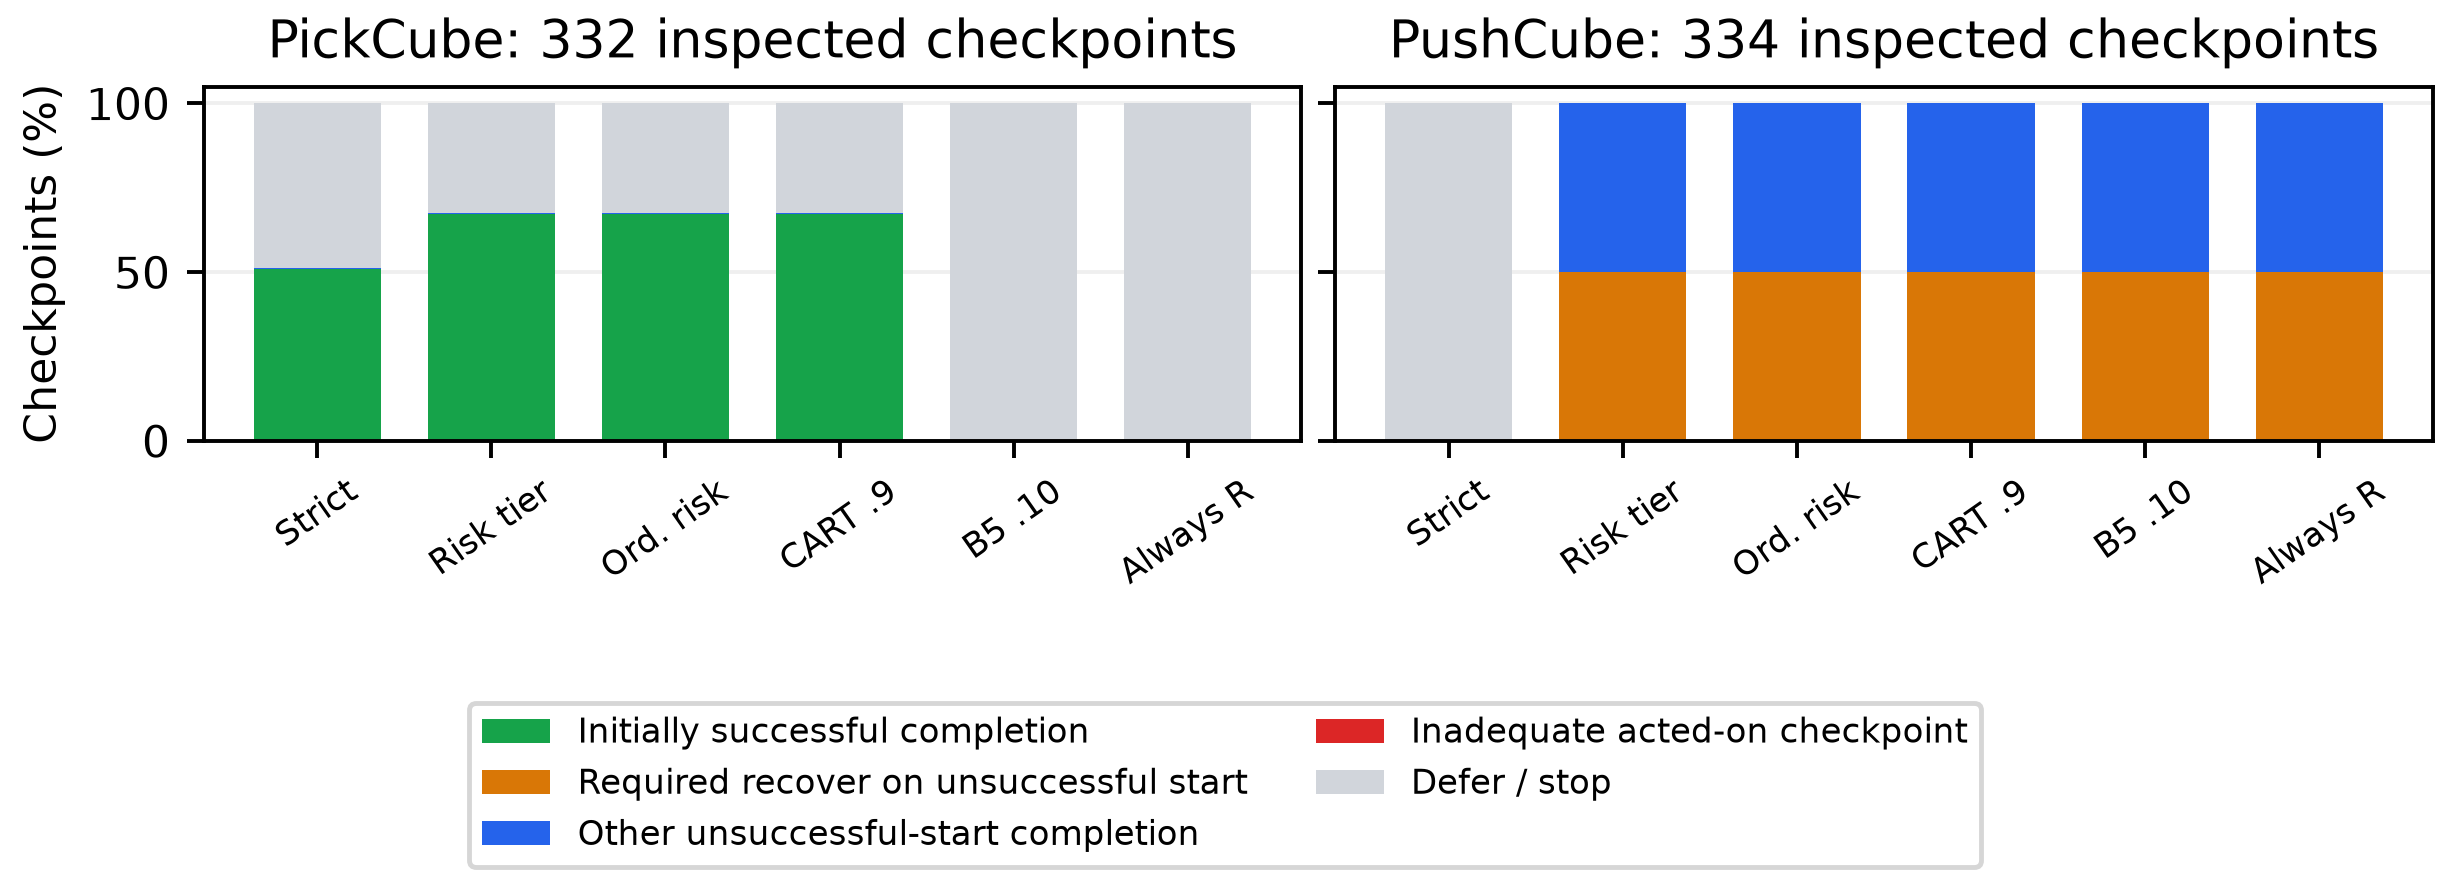
\includegraphics[width=\textwidth]{figures/operational.png}
\caption{Inspected historical follow-up under newly calibrated gates; exploratory, not new test. Deferral is explicit zero autonomous completion. Maintained success, required recovery and other initially unsuccessful completion are different outcomes; initially unsuccessful does not imply an annotated failure event. Ordinary B7 risk is equivalent. No gain is attributed to a new controller.}
\label{fig:operational}
\end{figure*}

No selected action was executed, so execution parity and its trajectory-error statistic are not assessable. The guard failure is retained as an engineering limitation, not evidence of physical nondeterminism.

\subsection{Imperfect observation and external validity}
The complete fixed corruption grid is an offline reanalysis of inspected inputs, not independent confirmation or an actual sensor deployment. Figure~\ref{fig:robustness} reports proposed successful and inadequate actions; all three noise replicates are averaged without changing the independent parent count. Factual contradictions, action/certificate stability, unavailable observations and the boundary-proximity subgroup delimit what the explanation assumes. A supplied fact can be wrong or stale even when the exact rule is correct. Clean risk eligibility is not transferred to corrupted packets, and retrospective telemetry checks are not an online fault detector.

\begin{figure*}[t]
\centering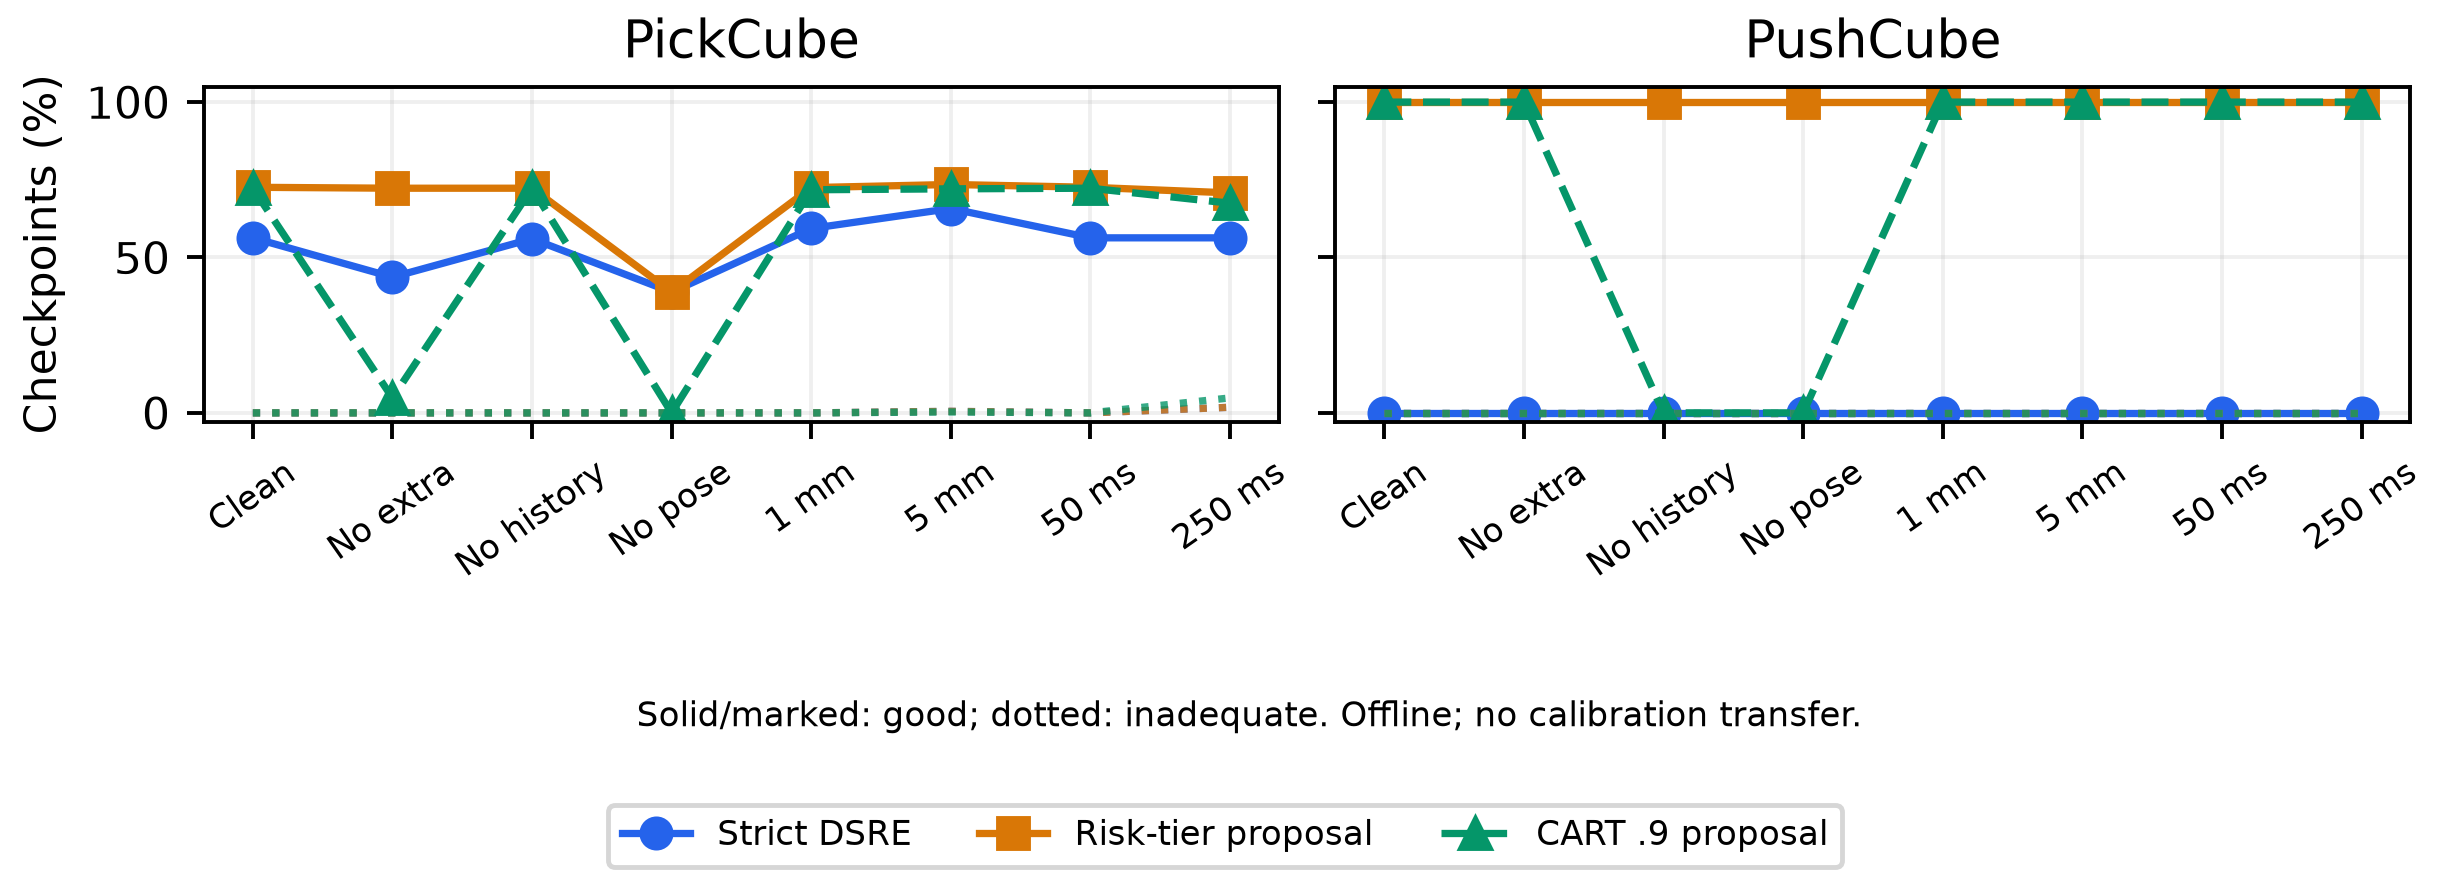
\includegraphics[width=\textwidth]{figures/observation_robustness.png}
\caption{Fixed offline observation sensitivity on the inspected 666-checkpoint follow-up. Marked curves show successful recommendations; dotted curves show inadequate actions. Noise points average three predeclared replicates; no additional independent parents or sensor hardware are claimed. Clean calibration is inapplicable under corruption. Full replicate and boundary results are reported separately.}
\label{fig:robustness}
\end{figure*}

The preselected Lift/Panda arm failed a source-semantic prerequisite before new physics: its existing alternative only clips nominal lift speed, and the retained 210 starts have no failure or varying-adequacy contrast. No new controller, fault or favorable replacement task was developed. Consequently distinct third-task recovery validation remains absent. This is a material breadth limitation, not a positive transfer finding.

Recorded clean observation histories contain 24 scalar fields, averaging 638.7 bytes for Pick and 620.2 for Push in compact JSON. All 17 methods together take mean 8.80 ms, median 0.0009 ms, p 950.0029 ms and maximum 276.99 ms per inspected checkpoint. Identical-query memoization makes these mixed cold/cached-call costs, not isolated method benchmarks or sensing/actuation latency. Boolean counts are representation cost, not sensor energy.

On the inspected Pick inputs, strict proposals have 187 good/0 inadequate choices clean, mean 218.3/1.7 under 5-mm noise and 187/6 under 250-ms delay; CART$.9$ has mean 239.3/1.0 under that noise and 224/16 under delay. Strict noise certificates assert a clean-telemetry-contradicted fact in mean 36.3 proposals, versus 34.0 for CART. These are fixed-replicate averages, not additional independent samples or a superiority guarantee. Pose-corrupted inputs can increase apparent coverage while invalidating factual evidence; retrospective contradictions are not online detection.

\section{Discussion and Remaining Scientific Boundaries}
The new held-out operational study is incomplete and cannot establish an independently tested completion gain. The risk bounds are independent calibration results; retrospective operational estimates cannot repair the missing test. Finite reference justification, measured action adequacy and independent statistical eligibility are different claims. Deferral has an explicit autonomy cost, and an adequate action need not be uniquely required. The operational comparison tests those consequences under identical information and error budgets. It does not create a new controller or make strict finite purity a population guarantee.

Exact B7 and the ordinary risk wrapper retain identical decisions and minimum facts. Selective classification and exact binomial risk control are established. Strong trees and constant policies may match or exceed a proposed operating point; all such comparisons remain in the same results. The candidate contribution is a robotics information contract and empirical characterization, not new pure-rule mathematics or calibration theory.

The parent-action confidence statement assumes independent seed-parent draws from the declared simulator distribution, two registered conditions, unchanged skills/horizon and a trustworthy clean observation interface. Grouping conditions prevents pseudoreplication; it does not prove distributional independence or transfer. Rare or absent actions remain unqualified; extra nominal continues cannot supply independent recovery assignments. The offline corruption experiment does not alter controller perception and cannot establish closed-loop sensor robustness. Retrospective factual diagnostics are not an online pose-health detector. No clean confidence bound transfers to noise, staleness or arbitrary checkpoints.

Two simple scripted tasks, idealized poses, deterministic branches, binary horizon-specific utility and the blocked Lift recovery contrast limit breadth. No real-hardware, human-interpretability or new sensor-cost claim is made. Remaining work requires a meaningful independently qualified third intervention, fixed independent rare-action cohorts and realistic observation validation, without inventing an algorithmic advantage. Formal manuscript completeness is separate from the significance judgment of RSS reviewers.

\clearpage
\bibliographystyle{plainnat}
\bibliography{operational_references}
\end{document}
